%%
%% THIS IS THE LaTeX RESEARCH PLAN TEMPLATE OF THE RESEARCH COUNCIL OF FINLAND FOR THE 2027 WINTER CALL: Academy Project Funding.
%%
%% THE STYLE AND HEADERS HAVE BEEN PRESET ACCORDING TO THE RESEARCH COUNCIL'S RULES. THE RESULTING PDF FILE OF THE RESEARCH PLAN WILL BE AUTOMATICALLY CHECKED WHEN UPLOADING IT. THE APPLICATION CANNOT BE SUBMITTED IF THE SYSTEM DETECTS AN DEVIATION IN THE HEADINGS, THE PAGE CONFIGURATION OR THE STRUCTURE OF YOUR RESEARCH PLAN PDF FILE. 
%%
\documentclass[a4paper,12pt]{article}

% Language support (including nordic letters)
\usepackage[T1]{fontenc}  
\usepackage[english]{babel}

% Math support
\usepackage[intlimits]{amsmath}
\usepackage{amsthm}

% Symbol support
\usepackage{amssymb}
\usepackage{eurosym}

% Image support and enabling wrapping of images
\usepackage[pdftex]{graphicx}
%\usepackage{wrapfig}

% Table extras support and using colors
\usepackage[table]{xcolor}
%\usepackage{booktabs}

% Item list extras for reduced spacing between items
\usepackage{enumitem}
\setlist{nosep}

% Hyperlink support (only for external hyperlinks) 
\usepackage{hyperref}
\hypersetup{
    colorlinks=true,
    urlcolor=cyan,
}

%% N.B. YOU MAY ALSO ADD YOUR OWN LaTeX PACKAGES HERE. NOTE THAT THE PACKAGES CANNOT BE IN CONFLICT WITH OR OVERRUN THE TEMPLATE SETTINGS SET BY THE RESEARCH COUNCIL OF FINLAND. 
\usepackage{array}
\usepackage{longtable} % lets the long tables break across pages
\usepackage{afterpage} % puts Fig. 1 at the top of page 2
\usepackage{tikz} % Table 1 is drawn with TikZ (text >= 10 pt)
\usetikzlibrary{arrows.meta}
% Drafting aid: red placeholder for facts still to be supplied (remove before submission)
\newcommand{\tbd}[1]{\textcolor{red}{[TBD: #1]}}
\newcommand{\doilink}[1]{\href{https://doi.org/#1}{doi:#1}} % clickable DOI in the reference list
\newcommand{\red}[1]{\textcolor{red}{#1}}
\definecolor{dkgreen}{RGB}{0,100,0}
\definecolor{dkorange}{RGB}{200,90,0}
\newcommand{\oc}[1]{\textcolor{dkorange}{#1}} % revision 3 (M7/M8 merged, monolithic heaters, second staff scientist): changed text in dark orange (remove before submission)
\definecolor{dkpurple}{RGB}{112,48,160}
\newcommand{\pc}[1]{\textcolor{dkpurple}{#1}} % revision 4 (final budget: DFG system, EBL batch, MSc months, research assistant): changed text in dark purple (remove before submission)
% revision 5 (SS 8 months, project-month labels, PhD2 m11--46, UiT 3 months): changed text in \red{red}
\definecolor{boxfill}{RGB}{221,230,245}
\definecolor{boxline}{RGB}{75,95,165}
%\hypersetup{citecolor=blue!50!black} % citation links in dark blue instead of hyperref's default light green
\hypersetup{citecolor=cyan} % citation links in dark blue instead of hyperref's default light green
\definecolor{dkteal}{RGB}{0,115,125}
\newcommand{\tc}[1]{\textcolor{dkteal}{#1}} % revision 6 (TAU advisors and co-supervisors, letters): changed text in dark teal (remove before submission)
\definecolor{dkmagenta}{RGB}{150,0,110}
\newcommand{\mc}[1]{\textcolor{dkmagenta}{#1}} % revision 7 (1 MEUR budget: postdoc, longer PhD contracts, breath pilot): changed text in dark magenta (remove before submission)
\definecolor{dkbrown}{RGB}{125,70,0}
\newcommand{\bc}[1]{\textcolor{dkbrown}{#1}} % revision 8 (no purchased fallback laser; PPLN-based source for broad coverage): changed text in dark brown (remove before submission)
\definecolor{dkolive}{RGB}{100,100,0}
\newcommand{\lc}[1]{\textcolor{dkolive}{#1}} % revision 9 (PhD2 36+6 months, m7--48; budget v5): changed text in dark olive (remove before submission)
\definecolor{dkrose}{RGB}{160,50,80}
\newcommand{\zc}[1]{\textcolor{dkrose}{#1}} % revision 10 (detector-noise budget): changed text in dark rose (remove before submission)
\definecolor{dkgray}{RGB}{90,90,90}
\definecolor{dkcyan}{RGB}{0,150,210}
\definecolor{dkleaf}{RGB}{40,170,30}
\definecolor{dkindigo}{RGB}{75,0,160}
\definecolor{dkplum}{RGB}{125,0,95}
\definecolor{dkrust}{RGB}{170,60,30}
\definecolor{dkmaroon}{RGB}{150,0,40}
\newcommand{\wc}[1]{\textcolor{dkmaroon}{#1}} % revision 20 (simulations at the M2 minimum R = 95 %: Figs. 2-3, Sec. 3.2, milestones and risks): changed text in maroon (remove before submission)
\newcommand{\jc}[1]{\textcolor{dkrust}{#1}} % revision 18-19 (10--30 mW idler plan with high-power pump lasers via R. Gumenyuk, M7 at 100 ms, M3/M6 specifications, ethane stretch goal, asthma pilot aligned with the letter of Prof. Lehtim\"aki): changed text in rust (remove before submission)
\newcommand{\hc}[1]{\textcolor{dkplum}{#1}} % revision 17 (wave-model results of QUIET Tasks 13-14: input phase-space and membrane-index dithers, 100 ms limits, new Figs. 2-3): changed text in plum (remove before submission)
\newcommand{\fc}[1]{\textcolor{dkindigo}{#1}} % revision 16 (Fig. 2f reconciled with the text, wave-bounded angle dither, honest chaotic gain): changed text in indigo (remove before submission)
\newcommand{\nc}[1]{\textcolor{dkleaf}{#1}} % revision 15: impact insertions (theory, consumable chip, methane and climate); remove before submission
\newcommand{\rc}[1]{\textcolor{dkcyan}{#1}} % revision 13 (cell-loss budget, idler power, averaging times): changed text in cyan (remove before submission)
\newcommand{\kc}[1]{\textcolor{dkgray}{#1}} % revision 12 (final budget: PhD2 40 months, SS 9 months, DFG detector line): changed text in dark gray (remove before submission)
\newcommand{\gc}[1]{\textcolor{dkgreen}{#1}} % workload-balance revision: changed text in dark green (remove before submission)
\newcommand{\chg}[1]{\textcolor{blue}{#1}} % revision for the DFG light source: changed text in blue (remove before submission)
\xdef\personpos{-7.4}
% Math in the main text font (Carlito): digits, Latin letters, minus and times signs, loaded after the template font package.
% Greek letters (Gamma, epsilon) stay in Computer Modern, because no Greek Carlito encoding exists for pdfLaTeX.
\usepackage{etoolbox}
\usepackage{cite} % compresses consecutive citation numbers, e.g. [17--20]
\AtEndPreamble{%
  \usepackage[italic,defaultmathsizes,unicodeminus]{mathastext}%
  \renewcommand{\times}{\mathbin{\text{\texttimes}}}%
}
 
%-----------------------------------------------------
% RESEARCH COUNCIL SETTINGS: DO NOT ALTER THESE SETTINGS! 
%-----------------------------------------------------

% Instruction text definition. 
\newcommand{\instructions}[1]{\textcolor{blue}{#1}}

% ONLY CALIBRI/CARLITO ARE ALLOWED AS FONT, FONT SIZE 12 PT DEFINED ABOVE. The font is used to ensure equal settings between LaTeX and Word templates.
% Find the font package here: https://www.ctan.org/tex-archive/fonts/carlito
\usepackage[sfdefault]{carlito}

% Linespacing 1 support and set space
\usepackage{setspace}
\singlespacing

% Page margin support and set page margins 20 mm
\usepackage[left=20mm, top=20mm, bottom=20mm, right=20mm]{geometry}

% Setting spacing for section, subsection and paragraph
\usepackage{titlesec}
\titleformat*{\section}{\large\bfseries}
\titleformat*{\subsection}{\bfseries}
\titlespacing{\section}{0 cm}{6pt}{0pt}
\titlespacing{\subsection}{0 cm}{6pt}{0pt}
\setlength{\parskip}{6pt}

%Aligning text to left
\raggedright

% Sets page numbers and header 
\usepackage{fancyhdr}
\pagestyle{fancyplain}
\fancyfoot{}
\fancyhead{}
\renewcommand{\headrulewidth}{0pt}
\rhead{\fancyplain{}{\thepage}({\pageref{lastpage}}) }

%-----------------------------------------------------

%%%%%%%%%%%%%%%%%%%%%%%%%%%%%%%%%%%%

\begin{document}

%% >>>>>>>>>> ADD YOUR RESEARCH PLAN TITLE IN THE FIELD BELOW:
%\textbf{\LARGE{QUIET: Quenching Unwanted Interference in Extended-path Trace-gas sensors}}\\
\textbf{\LARGE{QUIET: Quenching Unwanted Coherence-induced Interference in Extended-path Trace-gas Sensors}}\\
\vspace{12pt}%Quenching coherence noise in chip-scale multipass cells for gas sensing
%% >>>>>>>>>> ADD YOUR NAME AND THE ABBREVIATION OF CONSORTIUM IF APPLICABLE:
{\fontsize{14pt}{14pt}\selectfont\textbf{Mikko Huttunen, Tampere University
}}
\vspace{6pt}
%%%%%%%%%%%%%%%%%%%%%%%%%%%%%%%%%%%%

\vspace{6pt}

\section{Background and significance} 

\subsection*{1.1 From breath diagnostics to chaotic multipass cells on an integrated photonic chip}

Exhaled breath is a non-invasive window into the body: its trace chemistry changes with diseases and disorders, during airway inflammation or due to cancer~\cite{Dweik2011,Haick2014}. Its ppb-level trace molecules, volatile organic compounds (VOCs) and small gases such as nitric oxide (NO), ammonia and ethane (C$_2$H$_6$), arise from metabolism, inflammation and infection \cite{Haick2014}. The best-established breath test is exhaled NO (FeNO), interpreted at 5--50 ppb for asthma \cite{Dweik2011}.
Gas chromatography with mass spectrometry (GC--MS) identifies hundreds of breath compounds but needs bulky instruments and trained operators, far from the point of care. Electronic noses do not provide molecular specificity. Optical absorption spectroscopy offers a third route: it is molecule-specific, calibration-friendly and real-time, with sensitivity set by absorption coefficient times path length (Beer--Lambert law). For example, on-chip absorption sensing has recently reached NO$_2$ and methane (CH$_4$) detection with a 210 ppb sensitivity at mid-IR (mid-IR) \cite{Fan2026}.

%Three obstacles remain. \textbf{Path length.} In single-mode waveguides the path is limited by sidewall-roughness loss and by the footprint of the folded waveguide: gas-equivalent paths are about 1 cm \cite{Zhao2022}, far from what ppb sensitivity needs. \textbf{Coherence.} Long paths in compact cavities produce etalon fringes and speckle, a dominant noise source in laser absorption spectroscopy \cite{Li2014}, and a known limiter of on-chip gas sensors \cite{Yan2024}. Remedies treat the symptom: background subtraction \cite{Li2014}, moving diffusers or low-coherence sources that cost resolution or power \cite{Lu2024}. \textbf{Wavelength.} The strongest lines of many VOCs, including CH$_4$ and C$_2$H$_6$, lie at 3--3.5\,\textmu{}m or beyond, outside the mature near-infrared platforms.
Three remaining obstacles are related to \textbf{path length}, \textbf{coherence}, and \textbf{wavelength}. In single-mode waveguides the path is limited by sidewall-roughness loss and by the footprint of the folded waveguide: gas-equivalent paths are about 1 cm \cite{Zhao2022}, far from what ppb sensitivity needs. Long coherent light paths in detection cells produce etalon fringes and speckle, a dominant noise source in laser absorption spectroscopy \cite{Li2014}, and a known limiter of on-chip gas sensors \cite{Yan2024}. Remedies treat the symptom: background subtraction \cite{Li2014}, moving diffusers or low-coherence sources that cost resolution or power \cite{Lu2024}. Finally, the strongest lines of many VOCs, including CH$_4$ and C$_2$H$_6$, lie at 3--3.5\,\textmu{}m or beyond, outside the mature near-infrared platforms.

\textbf{Research question.} \emph{Can chaotic multipass cells (technology developed during QUIET) provide, on a single chip, (i) \textbf{long effective path lengths} in a compact footprint, (ii) intrinsic \textbf{suppression of coherence-induced noise}, and (iii) \textbf{mid-IR access} to the 3--3.5\,\textmu{}m band --- and together enable multi-species VOC detection at ppb levels at the point of care?}

We address the three obstacles with one concept. Light propagation in multimode slab-mode cells decouples path length from waveguide loss and footprint. Modulation of the properties of light (wavelength and propagation paths) randomizes the interference patterns along independent dimensions, so fringe- and speckle-noise average out. Cell design and instrumentation development allows extending detection from 1.5\,\textmu{}m to 3--3.5\,\textmu{}m, where the strongest VOC lines reside.

%\textbf{How QUIET goes beyond SOTA.} Free-standing on-chip waveguides achieve about 20\,ppb of CO$_2$ and 300\,ppb of CH$_4$ sensitivity \cite{Salaj2024,Jagerska2023}, but are limited by loss and footprint to gas-equivalent paths of ${\sim}$1\,cm \cite{Zhao2022}. Compact bulk cells with interband cascade lasers reach 5--8\,ppb of CH$_4$ and C$_2$H$_6$ with tens of metres of path in about 10\,cm \cite{Dong2016}, and laboratory cavity methods about 0.1\,ppb of ethane in breath \cite{Dahnke2001}. QUIET aims at compact-bulk sensitivity in a millimetre-scale, passive, batch-fabricated cartridge with the noise suppressed in the cell; only the 2\,ppb ethane goal goes beyond.

\textbf{How QUIET goes beyond SOTA.} Free-standing on-chip waveguides achieve about 20\,ppb of CO$_2$ and 300\,ppb of CH$_4$ sensitivity \cite{Salaj2024,Jagerska2023}, but are limited by loss and footprint to gas-equivalent paths of ${\sim}$1\,cm \cite{Zhao2022}. Compact bulk cells (with ${\sim}10$ m of path folded into 10\,cm cell) reach 5--8\,ppb of CH$_4$ and C$_2$H$_6$ \cite{Dong2016}, while bulk cavities reach ${\sim}$0.1\,ppb of C$_2$H$_6$ in breath \cite{Dahnke2001}. %QUIET aims at similar sensitivities in millimetre-scale devices, enabling dynamic detection of VOCs, CH$_4$ and C$_2$H$_6$ during breathing process.
QUIET aims at similar sensitivities in a millimetre-scale cartridge at 100 ms time resolution, so that changes in breath CH$_4$, C$_2$H$_6$ and VOC concentrations could be detected dynamically during a single exhalation process. 

% Fig. 1 is placed at the top of the page after this one (visual overview of the devices)
%\afterpage{%
\begin{figure}[t]
\centering
\includegraphics[width=\linewidth]{figs_new/Fig1_combined_setup_vector.pdf}
\raggedright\small \textbf{Figure 1.} Overview of the on-chip gas sensors. (a) Segmented CMPC and (b) Herriott cell on a free-standing membrane, with in-plane DBR facets, an input grating port (yellow) and output ports (blue). Red lines are ray paths. (c) Gas is sensed via evanescent fields of guided modes (decay length $\delta$). (d) E-field-weighted gas confinement factor $\Gamma$ versus thickness $t$ of SiN$_x$ membranes at 1.55\,\textmu{}m (solid) and 3.3\,\textmu{}m (dashed). The dot marks the 500 nm (1000 nm) SiN$_x$ design at 1.55\,\textmu{}m (3.3--3.4\,\textmu{}m). (e) Sensor device. Reusable reader, I: source (tunable narrow-linewidth laser, driving electronics, beam scanner for the angle and position dithers) and III: detection (detectors $1\ldots N$, reference R). Single-use cartridge, II: passive CMPC chip with a wide input grating port, output couplers and a reference channel in a gas-tight holder with windows and gas ports. %Component graphics: A.~Franzen, ComponentLibrary (CC BY-NC 3.0).
\end{figure}%}


\subsection*{1.2 Aim and research objectives}

The aim of QUIET is to show that chaotic multipass cells with dithered single-port injection enable chip-scale gas sensing with long effective path lengths and minimal coherence noise --- and to bring this sensing platform to the mid-IR lines needed for analyzing breath VOCs, with a proof-of-principle breath measurement. 
Three research objectives (ROs) address the obstacles standing our way.
%Three research objectives (ROs) address the obstacles of Sec.~1.1: coherence, path length and wavelength. 

\underline{\textbf{RO1: Suppress coherence noise.}} \emph{\textbf{Challenge}:} long optical paths are conventionally folded in multipass cells whose ray dynamics are regular: the rays close on themselves and visit only a few discrete path lengths (Fig.~2) \cite{White1942,Herriott1964}. Consequently, coherent interference appears as periodic fringes, and in on-chip cells as speckle patterns limiting the sensitivity. Fast laser frequency dithering (or modulation) solves this in bulk multipass cells --- but is hard to translate to on-chip sensors, and reduces the spectral resolution, creating a resolution vs.~sensitivity compromise.

%\emph{\textbf{Objective}:} establish a theory and design framework for chaotic multipass cells, where rays/beams mix over a continuous range of path lengths and angles (Fig.~2). The framework links the path-length and angle statistics to the coherence noise and the detection limit. It also uses the multimode nature of the cell as a new degree of freedom. \hc{Beams launched at different angles and positions through a wide grating port sweep independent input states (\textbf{input dithering}), and a thermo-optic modulation of the membrane index changes the optical paths inside the cell (\textbf{$\delta n$ dithering}); neither moves the laser line, so both add averaging dimensions to spectral dithering and preserve the spectral resolution \cite{Redding2012,Cao2019}.}
\emph{\textbf{Objective}:} establish a theory and design framework for chaotic multipass cells, where rays/beams mix over a range of varying path lengths (Fig.~2). The framework links the path-length and beam trajectories to the coherence noise and the detection limit. It also uses the multimode nature of the cell as a new degree of freedom. Beams launched at different angles and positions into the cells sweep independent input states (\textbf{input dithering}), while thermo-optic modulation of the membrane refractive index changes the optical paths inside the cell (\textbf{$\delta n$ dithering}). As these dithering methods do not modulate the laser frequency, coherence-induced speckle noise is reduced while preserving the spectral resolution \cite{Redding2012,Cao2019}.

\emph{\textbf{Hypothesis}:} in chaotic cells each added dither dimension (wavelength, input angle and position, membrane index) multiplicatively lowers the residual fringe noise, following an inverse square root of the number of swept input states. The hypothesis fails if the input (angle + position) or $\delta n$ dither does not lower the measured fringe beyond the wavelength dither alone\red{, or if a regular cell of equal footprint does equally well over the dither depths and film thicknesses of the fabricated chips}. Preliminary wave simulations support my hypothesis (Fig.~2f, Sec.~3.2).

%\emph{\textbf{Hypothesis}:} in chaotic cells each added dither dimension (wavelength, input angle and position, membrane index) multiplicatively lowers the residual fringe noise, following an inverse square root of the number of swept input states, to below $5\times10^{-7}$ with all of them. The hypothesis fails if the input or $\delta n$ dither does not lower the measured fringe beyond the wavelength dither alone, or if a regular cell of equal footprint does equally well over the dither depths and film thicknesses of the fabricated chips. Preliminary wave simulations support the first part (Fig.~2f, Sec.~3.2).

\begin{figure}[!t]
\centering
\includegraphics[width=\linewidth]{figs_new/Fig2_CMPC_sensors_vector.pdf}
\raggedright\small \textbf{Figure 2.} \hc{Preliminary simulations (Sec.~3.2) of regular and chaotic cells (RO1, RO2). (a,b) Segmented circular multipass cells, regular (R-CMPC) and chaotic (C-CMPC, 4\,mm, 16 index inclusions, orange dots), ray traces. (c,d) Herriott cells, regular (R-Herriott) and chaotic (C-Herriott). (e) Poincar\'e sections (angle of incidence $\chi$, position along the wall $s$). (f) Static residual fringe $\Delta P/P$ ($=2\sqrt{\varepsilon}\,V/\sqrt{M}$, with $V$ the fringe visibility and $M$ the number of speckle grains averaged by the detector) of 10\,mm cells with 8 inclusions (r 25\,\textmu{}m, $|\Delta n|$ 0.01) at 3.3\,\textmu{}m ($n_\mathrm{eff}=1.43$, $\Gamma=0.55$, \wc{$R=95\,\%$ (the M2 minimum)}, 0.3\,dB/cm, $\varepsilon=10^{-6}$), with the dithers added one by one: none, wavelength ($\lambda$, $\pm81$ pm), input angle ($\pm60$ mrad), input position ($\pm100$\,\textmu{}m, 75\,\textmu{}m beam on a grating port) and membrane index ($\delta n_\mathrm{eff}=10^{-4}$). Wave-consistent beamlet model; chaotic cells: medians of 30 inclusion layouts with interquartile whiskers; regular cells: single values, indicative only. Target $5\times10^{-7}$ (dashed line).}
\end{figure}

%\underline{\textbf{RO2: Chips with long path lengths.}} \emph{\textbf{Challenge}:} chip-based sensors detect gases through the evanescent fields of guided modes (Fig.~1c). In single-mode waveguides the gas-equivalent path stays near a centimetre \cite{Zhao2022} (Sec.~1.1), which keeps detection limits well above the ppb levels needed.
%
%\emph{\textbf{Objective}:} with our collaborators in UiT Tromsø, we will realise free-standing membrane cells with in-plane mirrors and a single-port fan-in (for dithering), and demonstrate on-chip noise suppression by using spectral and angle dithering. Main objective is to demonstrate sensing of breath-relevant analytes (ammonia, methane and ethane; Fig.~3a). Free-standing membranes have no etched sidewalls and large overlap of the optical field with the gas can be realized (Fig.~1d). Furthermore, a two-dimensional cell folds a long path (1–10 cm) into a very compact footprint of few millimetres, while entirely avoiding the need to realize lossy waveguide bends, in the multimode spirit of speckle spectrometers on disordered chips \cite{Redding2013} and light in complex media \cite{RotterGigan2017} (Fig.~1a,b,e). Our technological objective is to demonstrate a novel waveguiding platform not strongly hindered by the usual compromise between low propagation losses, and strong field overlap within the gas medium.
%
%\emph{\textbf{Hypothesis}:} propagation loss can be reduced by avoiding etched sidewalls. In etched channel waveguides, scattering from sidewall roughness is a dominant loss. In a free-standing membrane the light spreads in the film plane and meets no etched sidewalls. The losses are thus set by absorption and by the membrane roughness~\cite{Worhoff2008}. We expect losses low enough for gas-equivalent paths of several centimetres in a cell of a few millimetres in size. The etched edges that remain, the in-plane distributed Bragg reflector (DBR) mirrors, scatter at every bounce and are accounted for through the mirror reflectivities. The low film loss is supported by the literature (etched SiN$_x$ channels already reach 0.06 dB/cm \cite{Ji2023}, which bounds the film loss from above at 1.5\,\textmu{}m). As existing data on slab waveguides in the mid-IR region (3--3.5\textmu{}m) is scarce, part of RO3 is to provide such data. %Characterization of the roughness-induced loss is the first task of the fabrication work, and whether chaos still pays off at lower mirror reflectivity is tested in the theory work.

\underline{\textbf{RO2: Chips with long path lengths.}}
\emph{\textbf{Challenge}:} chip-based sensors detect gases through the
evanescent fields of guided modes (Fig.~1c). In single-mode waveguide gas sensors the path is limited by propagation loss and by the footprint of a folded waveguide, so the gas-equivalent path stays ${\sim}1$ cm \cite{Zhao2022}. This keeps sensitivities above the ppb levels needed for breath analysis.

\emph{\textbf{Objective}:} we will realize free-standing membrane cells with in-plane mirrors and a single wide grating input port (no electrical parts on the sensing chip) by two routes. First, via in-house fabrication working jointly with collaborators at UiT Tromsø, enabling fast prototyping and device development. Second, using commercial SiN$_x$ membranes patterned in-house by electron-beam lithography (EBL), laser ablation and by commercial EBL services (Applied Nanotools Inc.), to test fabrication scale-up. Spectral, input and $\delta n$ dithering will be demonstrated for noise suppression, with input dithering applied by a reusable reader outside the chip, so that the chip stays passive and suited to single use. The membrane has no lossy bends and supports many modes, as in multimode speckle-based spectrometers on disordered chips \cite{Redding2013} and light in complex media \cite{RotterGigan2017} (Fig.~1a,b,e). We will demonstrate (i)
gas-equivalent paths of 1--10~cm in cells a few millimetres across, and (ii) sensing of breath-relevant analytes
(methane and ethane, Fig.~3a).

\emph{\textbf{Hypothesis}:} a free-standing membrane avoids the current trade-off between low propagation loss and strong field overlap with the gas. Avoiding sidewall etching, the loss is set by film absorption and surface roughness, and is lower than in channel waveguides from the same film (0.11 versus 0.21 dB/cm for sputtered Al$_2$O$_3$ at 1.5\,\textmu{}m \cite{Worhoff2008}). %\red{slab-mode loss at 3--3.5\,\textmu{}m has, to our knowledge, not been reported.} 
Etched SiN$_x$ channels already reach losses <0.06~dB/cm \cite{Ji2023}, so with $\Gamma>40$\,\% (Fig.~1d) and mirror reflectivities above 95\,\% (target \red{97}\,\%) we expect gas-equivalent paths of several cm in a cell of a few mm in diameter\wc{ (simulated at $R=95\,\%$: $\Gamma\langle L\rangle$ 5.8 cm in a 5\,mm cell and 11 cm in a 10\,mm cell, Sec.~3.2)}. The hypothesis fails if the slab-mode loss exceeds 0.5~dB/cm. %(M2: 0.3~dB/cm). %A second hypothesis is that commercial membranes come within a factor of two of the in-house slab-mode loss and mirror reflectivity; it fails above 0.5~dB/cm.

\begin{figure}[!t]
\centering
\includegraphics[width=\linewidth]{figs_new/Fig3_CMPC_Spectroscopy.pdf}

\raggedright\small \textbf{Figure 3.} Simulated spectroscopy in breath background (RO1 and RO3). (a) Absorption coefficient of 1 ppm of \nc{CH$_4$ (1.64 and 3.31\,\textmu{}m) and C$_2$H$_6$ (3.34\,\textmu{}m)} in a breath background (grey), retrieved after averaging for \nc{100 ms} without dither (grey line) and with \hc{all dithers} (black). (b) Noise-equivalent absorbance \nc{(left) and CH$_4$ concentration (right) at the 3.31\,\textmu{}m line} versus averaging time $T$ \hc{without dither, with the wavelength ($\lambda$) or the input (angle + position) dither, with both, and with all dithers including the membrane-index modulation (black: total; blue: its fringe part; dashed: detector, 10 mW, NEP 14 pW/$\sqrt{\mathrm{Hz}}$, simulated transmission + 8 dB couplers). \wc{All dithers reach 2.2 ppb at 100 ms (1.4 ppb at $R=97\,\%$).} The cell is the 10\,mm chaotic CMPC of Fig.~2f (\wc{$R=95\,\%$}, $\Gamma\langle L\rangle\approx11$ cm), averaging locked to the dither periods, fringe drift 0.1 rad/s; medians and min--max bands of 30 inclusion layouts.}
\end{figure}

\underline{\textbf{RO3: Reach the mid-IR.}} \emph{\textbf{Challenge}:} the strongest VOC lines lie in the mid-IR, beyond the mature near-infrared platforms.

\emph{\textbf{Objective}:} stage the design from a near-infrared proof of principle (RO2) to mid-IR cells made in-house and from commercial SiN$_x$ membranes in parallel. Demonstrate multi-species sensing of methane and ethane (Fig.~3a), including a proof-of-principle measurement on human breath. Verify that the designs and the speckle reduction transfer also to the longer wavelengths. A tunable 3--3.5\,\textmu{}m source will be built in-house utilizing difference-frequency generation (DFG) in MgO:PPLN crystal, using a 1064\,nm pump laser and a tunable telecom laser.

\emph{\textbf{Hypothesis}:} because the lines are much stronger in the mid-IR, the speckle-limited detection limit of the same cell falls by roughly the same factor (Fig.~3), to the low-ppb range at equal path and noise, provided that both dithers and thermal stabilization are applied. The hypothesis fails if, at equal path, noise and averaging time, the mid-IR limit is less than 10 times below the near-infrared one (the M7 minimum). %\chg{ and that the DFG source gives enough idler power at low noise for the lossy cells (expected 0.1--10\,mW)}. %\red{Nitric oxide, the FeNO marker, lies at still longer wavelengths and is left to a follow-up.}

\textbf{From objectives to work packages.} RO1 is addressed in WP1 (theory, simulation and dither design), RO2 in WP2 (passive membrane cells with mirrors and a wide grating port, and their loss, reflectivity, path and speckle statistics), and RO3 in WP3 (gas-phase demonstration with the DFG source in the near- and mid-IR). WP4 (management, IP, reporting) is led by the PI. %The two doctoral students share the work along two lines: PhD student 1 the device and cavity, and PhD student 2 the dither and sensing (fan-in and angle dither, detection limits, gas measurements). Both work in the cleanroom.

\section{Impact}

\subsection*{2.1 Scientific impact}
\textbf{Core result: a coherence-noise law.} The central scientific product of QUIET is a theory that predicts the residual coherence noise of a multipass cell from its ray statistics alone. The path-length distribution $p(L)$ sets the spectral correlation $C(\Delta\lambda)$ and thus the number of independent patterns $N_\lambda$; launch angles and positions add $K$ more, and the noise falls as $(KN_\lambda)^{-1/2}$. The law does not depend on geometry, material or wavelength, so it applies to any passive mixing cavity, and it is testable: M3 compares the measured residual fringe with the prediction. \hc{In preliminary wave simulations of a 10\,mm chaotic cell each dimension lowers the fringe: the wavelength dither 20-fold, the input dither 11-fold (following the inverse square root of its $\approx$86 input states), the membrane-index modulation another 10-fold (Sec.~3.2).} Chaotic and random cavities are known to lower source coherence for speckle-free imaging \cite{Redding2012,Cao2019}, but to our knowledge no quantitative treatment links the path-length statistics of a wave-chaotic cavity to the residual fringe noise of absorption spectroscopy; the $1/\sqrt{M}$ speckle-contrast law \cite{Goodman2020} is our starting point, extended to angle, position and wavelength.

\textbf{Expected results} (milestones in Sec.~3.1). \emph{\textbf{RO1}:} the law above, demonstrated on chaotic multipass cells. \emph{\textbf{RO2}:} the first fabricated cells, with measured reflectivity, slab-mode loss and a reproducible process, testing the central hypothesis of a several-centimetre gas-equivalent path in a 3--5\,mm cell. \emph{\textbf{RO3}:} a tunable 3.06--3.66\,\textmu{}m DFG source built from existing lasers (M6), the first slab-mode loss data at 3--3.5\,\textmu{}m, a detection limit of 10 ppb or better for methane or ethane \jc{at 100 ms averaging} (2 ppb for ethane as a stretch goal), simultaneous retrieval of at least three species, and \jc{proof-of-principle breath measurements in healthy volunteers and about 20 asthma patients against a reference method and exhaled nitric oxide (FeNO)}.

%\textbf{Novelty and breakthrough potential.} Here coherence suppression is a property of the cell geometry and of its multi-mode, dithered excitation through a single input port. Proposed angle dithering (possible only in multimode systems) keeps the loss of spectral resolution small. If the hypotheses of RO1--RO3 hold, multi-species absorption sensing at ${\sim}$1-10 ppb levels becomes feasible on a chip, without moving parts, from 1.5 to 3.66\,\textmu{}m. This would be a technological breakthrough, demonstrating capabilities not existing in current sensing platforms, using a fabrication platform enabling mass-production of low-cost breath sensors usable directly at the point of care.  

\textbf{Novelty and breakthrough potential.} Existing remedies treat the symptom: they subtract the background, move a diffuser, or trade resolution or power for sensitivity. In QUIET the suppression is built into the cell: the chaotic geometry and multimode, dithered excitation randomize the interference pattern at the source, \hc{and the noise is averaged along independent dimensions: the wavelength, the input angle and position (possible only in a multimode cell) and the index of the guiding membrane itself. The last is specific to the chip: in a free-space cell the medium is the gas and path modulation needs moving mirrors, whereas the whole optical path of a membrane cell lies in a thin solid film whose index a CW pump or a heater swings by $10^{-4}$ within milliseconds, without moving parts. Input and index dithering leave the laser line fixed, so the resolution is preserved.} If RO1--RO3 hold, a single passive chip would combine the ppb limits of compact bulk sensors \cite{Dong2016} with a millimetre footprint and batch fabrication, which to our knowledge no chip platform offers. With the dithers applied by a reusable reader, the chip becomes a low-cost consumable (Sec.~2.2).

%The project demonstrates the concept at chip level; the millimetre-scale footprint and the use of standard microfabrication steps leave the route to batch fabrication and low-cost point-of-care breath sensors open.

%\textbf{Impact within the scientific community.} The design rules, the open simulation code and the measured speckle statistics will be published open access in at least eight articles (10 as target), and should transfer to other chip-scale interferometric and speckle-based sensors \cite{Redding2013}. Two doctoral students, a postdoctoral researcher, three MSc thesis students, and 1--3 BSc thesis students will be trained into the field that combines wave chaos, integrated photonics and gas spectroscopy. The postdoc and PhD2 will also be trained in nonlinear optics and mid-IR lasers. With the staff scientist, who documents the fabrication process, they form a local team that keeps this know-how at Tampere University (TAU). The DFG source adds a lasting tunable mid-IR laser capability at Tampere beyond QUIET.

\textbf{Impact within the scientific community.} Coherence noise limits every long-path integrated sensor, so the design rules, open code and measured speckle statistics (at least eight open-access articles, ten as target) transfer to integrated speckle spectrometers \cite{Redding2013}, speckle-based optical computing \cite{Arola2026} and fringe-limited bulk instruments. They give the wave-chaos community a quantitative link between cavity geometry and spectroscopic noise, and the integrated-photonics community a route to the mid-IR that does not depend on low-loss single-mode waveguides. QUIET trains two doctoral students, a postdoctoral researcher and MSc and BSc students in this combination of skills (Sec.~3.4), and the DFG source leaves a lasting tunable mid-IR capability at TAU.

\subsection*{2.2 Impact beyond academia}

\textbf{Need and benefit.} Many diseases are diagnosed late because tests are invasive, laboratory-based or effort-dependent. Exhaled breath carries markers of airway inflammation and metabolism at ppb levels \cite{Dweik2011}. \jc{Asthma is the lead clinical case: exhaled nitric oxide is measured with commercial devices, but only this one molecule, whereas the chip adds several (e.g.\ ethane) and, at 100 ms resolution, their time course within one exhalation.} A chip-scale sensor that quantifies several at once would bring breath tests to primary care, pharmacies and homes, enabling monitoring and screening.

\textbf{Route to use.} \nc{The cell is passive: the reader applies the angle and position dithers (T1.2), so the chip is a consumable like a test strip, single-use for breath tests, while laser, scanner and detectors stay in the reader. Single use removes cross-contamination and fouling. A 3--5 mm cell allows about 500--2\,000 chips per wafer; at 1--7\,k\texteuro{} per processed wafer (foundry quote in T4.2) this is about 0.5--15\,\texteuro{} per chip before packaging.} A point-of-care device would use a compact fixed-wavelength laser, e.g.\ an interband cascade laser at 3.3\,\textmu{}m. Intellectual property, in particular the dithering scheme, will be assessed with TAU innovation services before publication, \nc{and exploitation planning starts in month 1 (T4.2). A} proof-of-principle breath measurement, \nc{including about 20 asthma patients,} is part of QUIET (T3.4); \nc{larger} clinical validation is the follow-up. The work supports SDG 3 (health), 9 (industry and innovation) \nc{and 13 (climate action)}.

\textbf{Second application: methane and climate.} Methane accounts for about 0.5\,$^\circ$C of the 1.07\,$^\circ$C of human-caused warming in 2010--2019 \cite{IPCC2021}. EU Regulation 2024/1787 sets ppm-level repair thresholds \cite{EUMethane2024}; QUIET addresses the complementary need for dense, cheap fence-line monitoring, where emissions appear as tens to hundreds of ppb over a background of about 1.9\,ppm \cite{Saunois2025}. Ethane identifies the source (ethane-to-methane molar ratios of 0, 1.8 and 9.6\,\% for microbial, low-ethane and high-ethane fossil sources \cite{Smith2015}), so a 100 ppb methane enhancement carries up to about 10 ppb of ethane.


\section{Implementation}

\subsection*{3.1 Work plan and schedule}
Below, each work package (WP) and task (T) is given with its duration (m = month) and main responsible persons (PhD1, PhD2, the postdoc, MSc thesis students MSc1--MSc4, staff scientist (SS) or the PI). PhD1 works for m1--m42, working on the in-house SiN$_x$ line (theory, cleanroom, mirrors, loss, mid-IR membranes). PhD2 works for \nc{m7--m48}, working on optics and the commercial route (dither, fs-laser structuring, outsourced cells, grating input, validation line), with a cleanroom introduction only. The postdoc  (m13--48) leads the laser-spectroscopy tasks: setting up the DFG source, the spectroscopy experiments and the proof-of-principle human breath measurements. \nc{Four} MSc theses, each partly paid by the project (2.5 months each, \nc{10} months in total), take over design work: \nc{MSc1 cartridge and gas handling, with Prof.~Panu Karjalainen (m5--11),} MSc2 \nc{input grating port design (m9--15), MSc3 reader-side beam scanner and optical coupling to the cartridge (m13--19)}, MSc4 DFG source design (m17--23). \nc{Each starts from a first-pass design by the PhD students, so a missing thesis delays but does not block the work.} %Fabrication and measurements stay with the PhD students and the SS. 
The SS (Dr.~Marika Janka), a permanent cleanroom staff member, leads fabrication development and trains both doctoral students. The project pays for 9 months of staff scientist time (2 months a year, 1 in the last year), shared between the SS, who develops the recipes, trains PhD1 and advises later, and Dr.~Piotr Ryczkowski, experienced in optical laboratory set-ups, who supports the postdoc with the DFG source (T3.2). Milestones: Table 1.

%The two doctoral students share the work along two lines: PhD student 1 the device and cavity (chaotic cell design, membrane and mirror process, loss, reflectivity and speckle characterization), and PhD student 2 the dither and sensing (fan-in and angle dither, detection limits, gas measurements). Both work in the cleanroom.
\begin{figure}[!ht]
\centering
\raggedright\small \textbf{Table 1.} Work packages (WPs), tasks (T), schedule, division of work and milestones M1--M8.
%, described in the text. Bars show task-level division of work. %MPC: multipass cell. Milestones: M1, M3 test RO1; M2, M4 test RO2; M5 tests RO2 (absolute limit) and RO1 (dither and chaos gain); M6--M8 test RO3.
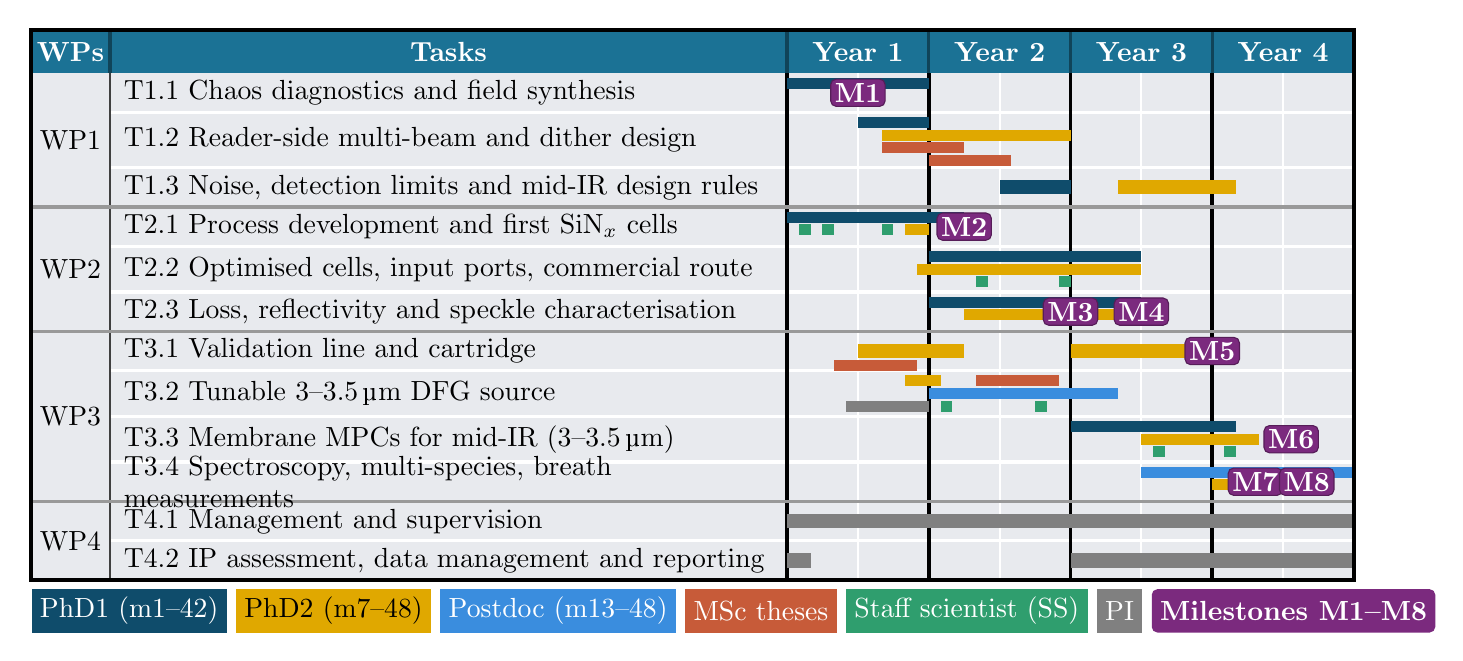
\begin{tikzpicture}[x=1cm,y=1cm,font=\fontsize{10}{11.5}\selectfont]
\hyphenpenalty=10000 \exhyphenpenalty=10000 \relax
\definecolor{phdcol}{HTML}{0F4C6B}\definecolor{pdcol}{HTML}{E0A800}\definecolor{picol}{HTML}{808080}\definecolor{sscol}{HTML}{2F9E6E}
\definecolor{thcol}{HTML}{C75B39}\definecolor{pdoccol}{HTML}{3A8DDE}
\definecolor{hdrcol}{HTML}{1B7295}\definecolor{bodycol}{HTML}{E8EAEE}\definecolor{mscol}{HTML}{7B2A7E}
\fill[bodycol] (0,-0.550) rectangle (16.80,-6.990);
\draw[white,line width=1.2pt] (1.00,-1.050) -- (16.80,-1.050);
\draw[white,line width=1.2pt] (1.00,-1.750) -- (16.80,-1.750);
\draw[white,line width=1.2pt] (1.00,-2.750) -- (16.80,-2.750);
\draw[white,line width=1.2pt] (1.00,-3.330) -- (16.80,-3.330);
\draw[white,line width=1.2pt] (1.00,-4.330) -- (16.80,-4.330);
\draw[white,line width=1.2pt] (1.00,-4.910) -- (16.80,-4.910);
\draw[white,line width=1.2pt] (1.00,-5.490) -- (16.80,-5.490);
\draw[white,line width=1.2pt] (1.00,-6.490) -- (16.80,-6.490);
\draw[white,line width=0.8pt] (10.500,-0.550) -- (10.500,-6.990);
\draw[white,line width=0.8pt] (12.300,-0.550) -- (12.300,-6.990);
\draw[white,line width=0.8pt] (14.100,-0.550) -- (14.100,-6.990);
\draw[white,line width=0.8pt] (15.900,-0.550) -- (15.900,-6.990);
\draw[black,line width=1.3pt] (9.600,-0.550) -- (9.600,-6.990);
\draw[black,line width=1.3pt] (11.400,-0.550) -- (11.400,-6.990);
\draw[black,line width=1.3pt] (13.200,-0.550) -- (13.200,-6.990);
\draw[black,line width=1.3pt] (15.000,-0.550) -- (15.000,-6.990);
\draw[black!75,line width=0.8pt] (1.00,-0.550) -- (1.00,-6.990);
\draw[black!40,line width=1.3pt] (0,-2.250) -- (16.80,-2.250);
\draw[black!40,line width=1.3pt] (0,-3.830) -- (16.80,-3.830);
\draw[black!40,line width=1.3pt] (0,-5.990) -- (16.80,-5.990);
\fill[phdcol] (9.600,-0.610) rectangle (11.400,-0.750);
\fill[phdcol] (10.500,-1.110) rectangle (11.400,-1.250);
\fill[pdcol] (10.800,-1.270) rectangle (13.200,-1.410);
\fill[thcol] (10.800,-1.430) rectangle (11.850,-1.570);
\fill[thcol] (11.400,-1.590) rectangle (12.450,-1.730);
\fill[phdcol] (12.300,-1.910) rectangle (13.200,-2.090);
\fill[pdcol] (13.800,-1.910) rectangle (15.300,-2.090);
\fill[phdcol] (9.600,-2.310) rectangle (11.850,-2.450);
\fill[sscol] (9.750,-2.470) rectangle (9.900,-2.610);
\fill[sscol] (10.050,-2.470) rectangle (10.200,-2.610);
\fill[sscol] (10.800,-2.470) rectangle (10.950,-2.610);
\fill[pdcol] (11.100,-2.470) rectangle (11.400,-2.610);
\fill[phdcol] (11.400,-2.810) rectangle (14.100,-2.950);
\fill[pdcol] (11.250,-2.970) rectangle (14.100,-3.110);
\fill[sscol] (12.000,-3.130) rectangle (12.150,-3.270);
\fill[sscol] (13.050,-3.130) rectangle (13.200,-3.270);
\fill[phdcol] (11.400,-3.390) rectangle (14.100,-3.530);
\fill[pdcol] (11.850,-3.550) rectangle (14.100,-3.690);
\fill[pdcol] (10.500,-3.990) rectangle (11.850,-4.170);
\fill[pdcol] (13.200,-3.990) rectangle (15.000,-4.170);
\fill[pdcol] (11.100,-4.390) rectangle (11.550,-4.530);
\fill[thcol] (10.200,-4.190) rectangle (11.250,-4.330);
\fill[thcol] (12.000,-4.390) rectangle (13.050,-4.530);
\fill[pdoccol] (11.400,-4.550) rectangle (13.800,-4.690);
\fill[picol] (10.350,-4.710) rectangle (11.400,-4.850);
\fill[sscol] (11.550,-4.710) rectangle (11.700,-4.850);
\fill[sscol] (12.750,-4.710) rectangle (12.900,-4.850);
\fill[phdcol] (13.200,-4.970) rectangle (15.300,-5.110);
\fill[pdcol] (14.100,-5.130) rectangle (15.600,-5.270);
\fill[sscol] (14.250,-5.290) rectangle (14.400,-5.430);
\fill[sscol] (15.150,-5.290) rectangle (15.300,-5.430);
\fill[pdoccol] (14.100,-5.550) rectangle (16.800,-5.690);
\fill[pdcol] (15.000,-5.710) rectangle (15.900,-5.850);
\fill[picol] (9.600,-6.150) rectangle (16.800,-6.330);
\fill[picol] (9.600,-6.650) rectangle (9.900,-6.830);
\fill[picol] (13.200,-6.650) rectangle (16.800,-6.830);
\node[fill=mscol,draw=mscol!70!black,rounded corners=2pt,text=white,inner sep=1.5pt,font=\fontsize{10}{11}\selectfont\bfseries] at (10.500,-0.800) {M1};
\node[fill=mscol,draw=mscol!70!black,rounded corners=2pt,text=white,inner sep=1.5pt,font=\fontsize{10}{11}\selectfont\bfseries] at (11.850,-2.500) {M2};
\node[fill=mscol,draw=mscol!70!black,rounded corners=2pt,text=white,inner sep=1.5pt,font=\fontsize{10}{11}\selectfont\bfseries] at (13.200,-3.580) {M3};
\node[fill=mscol,draw=mscol!70!black,rounded corners=2pt,text=white,inner sep=1.5pt,font=\fontsize{10}{11}\selectfont\bfseries] at (14.100,-3.580) {M4};
\node[fill=mscol,draw=mscol!70!black,rounded corners=2pt,text=white,inner sep=1.5pt,font=\fontsize{10}{11}\selectfont\bfseries] at (15.000,-4.080) {M5};
\node[anchor=west,fill=mscol,draw=mscol!70!black,rounded corners=2pt,text=white,inner sep=1.5pt,font=\fontsize{10}{11}\selectfont\bfseries] at (15.650,-5.200) {M6};
\node[anchor=east,fill=mscol,draw=mscol!70!black,rounded corners=2pt,text=white,inner sep=1.5pt,font=\fontsize{10}{11}\selectfont\bfseries] at (15.900,-5.740) {M7};
\node[fill=mscol,draw=mscol!70!black,rounded corners=2pt,text=white,inner sep=1.5pt,font=\fontsize{10}{11}\selectfont\bfseries] at (16.200,-5.740) {M8};
\fill[hdrcol] (0,0.000) rectangle (16.80,-0.550);
\node[text=white,font=\fontsize{10}{11.5}\selectfont\bfseries] at (0.50,-0.280) {WPs};
\node[text=white,font=\fontsize{10}{11.5}\selectfont\bfseries] at (5.30,-0.280) {Tasks};
\node[text=white,font=\fontsize{10}{11.5}\selectfont\bfseries] at (10.50,-0.280) {Year 1};
\node[text=white,font=\fontsize{10}{11.5}\selectfont\bfseries] at (12.30,-0.280) {Year 2};
\node[text=white,font=\fontsize{10}{11.5}\selectfont\bfseries] at (14.10,-0.280) {Year 3};
\node[text=white,font=\fontsize{10}{11.5}\selectfont\bfseries] at (15.90,-0.280) {Year 4};
\draw[hdrcol!60!black,line width=1.2pt] (1.00,0.000) -- (1.00,-0.550);
\draw[hdrcol!60!black,line width=1.2pt] (9.60,0.000) -- (9.60,-0.550);
\draw[hdrcol!60!black,line width=1.2pt] (11.40,0.000) -- (11.40,-0.550);
\draw[hdrcol!60!black,line width=1.2pt] (13.20,0.000) -- (13.20,-0.550);
\draw[hdrcol!60!black,line width=1.2pt] (15.00,0.000) -- (15.00,-0.550);
\node[font=\fontsize{10}{11.5}\selectfont] at (0.50,-1.400) {WP1};
\node[font=\fontsize{10}{11.5}\selectfont] at (0.50,-3.040) {WP2};
\node[font=\fontsize{10}{11.5}\selectfont] at (0.50,-4.910) {WP3};
\node[font=\fontsize{10}{11.5}\selectfont] at (0.50,-6.490) {WP4};
\node[anchor=west,text width=8.35cm,align=left,inner sep=2pt] at (1.10,-0.800) {T1.1 Chaos diagnostics and field synthesis};
\node[anchor=west,text width=8.35cm,align=left,inner sep=2pt] at (1.10,-1.400) {T1.2 Reader-side multi-beam and dither design};
\node[anchor=west,text width=8.35cm,align=left,inner sep=2pt] at (1.10,-2.000) {T1.3 Noise, detection limits and mid-IR design rules};
\node[anchor=west,text width=8.35cm,align=left,inner sep=2pt] at (1.10,-2.500) {T2.1 Process development and first SiN$_x$ cells};
\node[anchor=west,text width=8.35cm,align=left,inner sep=2pt] at (1.10,-3.040) {T2.2 Optimised cells, input ports, commercial route};
\node[anchor=west,text width=8.35cm,align=left,inner sep=2pt] at (1.10,-3.580) {T2.3 Loss, reflectivity and speckle characterisation};
\node[anchor=west,text width=8.35cm,align=left,inner sep=2pt] at (1.10,-4.080) {T3.1 Validation line and cartridge};
\node[anchor=west,text width=8.35cm,align=left,inner sep=2pt] at (1.10,-4.620) {T3.2 Tunable 3--3.5\,\textmu{}m DFG source};
\node[anchor=west,text width=8.35cm,align=left,inner sep=2pt] at (1.10,-5.200) {T3.3 Membrane MPCs for mid-IR (3--3.5\,\textmu{}m)};
\node[anchor=west,text width=8.35cm,align=left,inner sep=2pt] at (1.10,-5.740) {T3.4 Spectroscopy, multi-species, breath measurements};
\node[anchor=west,text width=8.35cm,align=left,inner sep=2pt] at (1.10,-6.240) {T4.1 Management and supervision};
\node[anchor=west,text width=8.35cm,align=left,inner sep=2pt] at (1.10,-6.740) {T4.2 IP assessment, data management and reporting};
\draw[black,line width=1.5pt] (0,0.000) rectangle (16.80,-6.990); 
\xdef\personpos{-7.38}
\node[name=lg0,anchor=west,fill=phdcol,text=white,inner sep=3pt,minimum height=0.55cm] at (0.00,\personpos) {PhD1 (m1--42)};
\node[name=lg1,anchor=west,fill=pdcol,text=black,inner sep=3pt,minimum height=0.55cm] at ([xshift=3pt]lg0.east) {PhD2 (m7--48)};
\node[name=lg2,anchor=west,fill=pdoccol,text=white,inner sep=3pt,minimum height=0.55cm] at ([xshift=3pt]lg1.east) {Postdoc (m13--48)};
\node[name=lg3,anchor=west,fill=thcol,text=white,inner sep=3pt,minimum height=0.55cm] at ([xshift=3pt]lg2.east) {MSc theses};
\node[name=lg4,anchor=west,fill=sscol,text=white,inner sep=3pt,minimum height=0.55cm] at ([xshift=3pt]lg3.east) {Staff scientist (SS)};
\node[name=lg5,anchor=west,fill=picol,text=white,inner sep=3pt,minimum height=0.55cm] at ([xshift=3pt]lg4.east) {PI};
\node[anchor=west,fill=mscol,text=white,inner sep=3pt,minimum height=0.55cm,rounded corners=2pt] at ([xshift=3pt]lg5.east) {\bfseries Milestones M1--M8};
\end{tikzpicture}
\end{figure}

\underline{\textbf{WP1: Theory, simulation and dither design}}

\textbf{T1.1 [Chaos diagnostics and field synthesis]:} \jc{We extend our Python tools (Sec.~3.2) to trace rays through a cell and compute the output interference pattern, and confirm with Poincar\'e sections and Lyapunov exponents that a cell is truly chaotic~\cite{CaoWiersig2015}. Circular and Herriott cells are regular by themselves, so we make them chaotic with small regions of different refractive index ($\Delta n\approx0.001$--0.01, Figs.~2b,d; in the membrane shallow-etched discs of 1--7 nm), a strong perturbation of the output speckle \cite{Arola2026}. We derive how the spread of path lengths, $p(L)$, sets the spectral correlation function $C(\Delta\lambda)$ \cite{CaoWiersig2015,Goodman2020} and test it against ray and wave simulations. Milestone M1 (m6): design framework validated, with the simulations of Fig.~2f extended to the fabricated geometry and $R=95$--99.5\,\%, and mirror specification agreed with WP2 (loss $\leq1\,\%$ per bounce, $R\geq99\,\%$ target; $\leq5\,\%$ minimum). If the chaotic cell does not beat the regular one under the same dithers (M5), regular cells are adopted; if the free-space analogue of T1.2 does not confirm the simulated number of independent patterns within a factor of two, the dither design is revised before the masks.} (PhD1, m1--12)

\textbf{T1.2 [Reader-side multi-beam angle, position and spectral dither design]:} \jc{The chip is a passive consumable, so the reader applies the dithers (Fig.~1e). We design a wide input grating port that maps the position and tilt of the incident beam to in-plane launch angles and positions, identical for both fabrication routes (PhD1 owns the design and signs off the masks by m15, with MSc2, m9--15), and the reader-side beam scanner, $\delta n$ pump and cartridge coupling (MSc3, m13--19). A free-space analogue (bulk chaotic cell at 1.5\,\textmu{}m, BSc student under the PI, m2--5, gate: M1) measures speckle decorrelation versus angle, position and wavelength before the masks. Launches give independent speckle only if the tilts exceed the beam divergence: the number of independent input states is waist $\times$ tilt $\times$ shift$/\lambda$, none for $\pm2$ mrad of a 40\,\textmu{}m beam and $\approx$86 at 3.3\,\textmu{}m for a 75\,\textmu{}m waist with $\pm60$ mrad and $\pm100$\,\textmu{}m (Sec.~3.2). The membrane index is modulated by a CW pump absorbed in the membrane or by heaters outside the beam paths ($\delta n_\mathrm{eff}=10^{-4}$, $\approx\pm9$ K at 20--50 Hz), with the readout averaged over whole periods. The spectral dither is applied to the telecom laser, also with the DFG source, and copied to the idler: $\pm81$ pm at 3.3\,\textmu{}m ($\pm2.2$ GHz) keeps 92\,\% of the CH$_4$ and 82\,\% of the C$_2$H$_6$ line peak.}

\textbf{T1.3 [Noise and detection limits, geometry choice and mid-IR design rules]:} \jc{Analysis of the noise floor and detection limit with all dithers (fringe, shot noise, drift; Fig.~3b) and comparison of the geometries in path, transmission and residual fringe; the working targets, fixed in year 1, are those of M5. The analysis is repeated at 3--3.5\,\textmu{}m for SiN$_x$ membranes (line strengths, speckle budget, thermal stabilization and the thermal side effects of the index modulation), giving the mid-IR chip design (RO3) and the predicted limits against which M7 is tested. Detector noise sets the averaging time $T$: $\delta=\sqrt{\mathrm{NEP}^2+2h\nu P_d}/(P_d\sqrt{2T})$, with $P_d$ the detector power. 10 ppb at 2 cm gas-equivalent path needs $\delta\approx6\times10^{-7}$, of which the detector may use $3\times10^{-7}$. The loss from idler to detector ($\Gamma\approx0.45$, ${\sim}$15 bounces) is ${\approx}$10--20 dB; we aim at 10--14 dB and accept 20--25 dB ($\Gamma\approx0.2$ or $R=90\,\%$). With the planned 10--30 mW idler (T3.2; 1 mW minimum) and an uncooled 14 pW/$\sqrt{\mathrm{Hz}}$ detector, 10 ppb needs $T\approx10$ ms at 14 dB and 0.1 s at 20 dB with 10 mW, and 0.1 s at 25 dB with 30 mW. \wc{The simulated 10\,mm cell at the M2 minimum $R=95\,\%$ (24 dB including the couplers, $\Gamma\langle L\rangle\approx11$ cm) reaches 10 ppb methane in 4 ms with 10 mW and in 0.4 s with 1 mW.} We state $T$ with every limit (M7 baseline 100 ms, up to 1 s).} (PhD1, m19--24; PhD2, m29--38)

\underline{\textbf{WP2: Fabrication and characterization}}

\textbf{T2.1 [Process development and first-generation SiN$_x$ cells]:} Development of the fabrication recipes for free-standing membranes, in-plane DBR mirrors and the release step at TAU. The SS owns the recipes and \nc{does the first process runs (m\nc{1--7}) while training PhD1, who takes over the runs from m\nc{8} after} a three-month visit to UiT Tromsø (J.~J\'agersk\'a, J.~Viljanen, m\nc{5--7}). First-generation SiN$_x$ Herriott-type cells with DBR mirrors are made jointly with UiT, and their reflectivity and loss are measured. From month 1, commercial SiN$_x$ membranes (e.g.\ Silson, Norcada) are bought and their planar loss and uniformity measured (T2.3), and test structures are cut by femtosecond-laser (fs-laser) ablation with existing fs lasers at TAU (PhD2, m11--12). Milestone M2 (m15): measured $R\geq 95\,\%$ (target 99\,\%\wc{; the simulations of Sec.~3.2 assume this minimum}) and slab-mode loss $\leq0.3$ dB/cm (target 0.1 dB/cm) at 1.5\,\textmu{}m, testing the loss hypothesis of RO2 on in-house and commercial membranes; the SS delivers a reproducible recipe. (SS, PhD1, Troms\o{}, m1--15; PhD2, m11--12)

\textbf{T2.2 [Optimised cells, \nc{input ports} and commercial route]:} In-house fabrication of \nc{passive} SiN$_x$ membrane cells with \nc{a wide input grating port and output couplers, without electrical parts,} at TAU (designs from T1.2). The SS adapts the recipes of T2.1 \nc{to the grating ports}; PhD1 makes membranes, mirrors \nc{and grating ports} (masks from MSc2 by m15, first run about m16, \nc{first coupling and speckle data at about m18, go/no-go on reader-side coupling at about m20}). \nc{All chips share one passive layout family with fixed outlines, so that the design transfers to lot-scale lithography (T4.2).} \emph{Commercial:} cell outlines are cut into commercial membranes by fs-laser ablation (PhD2), and one prototype batch of about 5 chips, with DBR mirrors and input and output grating couplers, is written by commercial EBL (Applied Nanotools, m20--28) after \nc{MSc2} has designed the gratings. The routes are compared by loss, reflectivity, speckle, yield and cost (T2.3). (PhD1, m13--30; PhD2, m12--30)

\textbf{T2.3 [Loss, reflectivity and speckle characterization]:} \jc{We measure mirror reflectivities, membrane losses and speckle statistics of regular and chaotic cells, with and without dither (including the membrane-index modulation), and compare them with the simulations. The slab-mode loss is also measured on planar membranes of the same film, in-house and commercial, separating film from mirror loss (RO2). Milestone M3 (m24), joint for both students: a ``stable CMPC'' on passive chips, with speckle statistics matching the simulated chaotic ensemble and a residual fringe below $5\times10^{-7}$ (minimum $5\times10^{-6}$) with reader-side angle, position, spectral and membrane-index ($\delta n$) dither (simulated \wc{$1.7\times10^{-7}$ at $R=95\,\%$}, and $1.6\times10^{-6}$ without $\delta n$, Fig.~2f), measured against reference detector R (noise floor below $10^{-7}$). It must hold for single use: at least 5 chips of one run, each inserted at least 3 times, with the fringe within a factor of 3. Milestone M4 (m30): a gas-equivalent path of at least 2 cm (minimum 1 cm) in a SiN$_x$ cell of 3--5 mm diameter at an insertion loss of at most 25 dB (goal 14 dB\wc{; simulated at $R=95\,\%$: 5.8 cm at 21 dB in a 5\,mm cell, including 8 dB for the couplers}), a commercial-membrane cell within a factor of two of this path, and a chip-to-chip path variation of at most 10\,\% (minimum 20\,\%), measured with a certified gas (T3.1), so that one calibration per lot suffices.} (PhD1, m13--30; PhD2, m16--30)

\underline{\textbf{WP3: Gas-phase demonstration and wavelength staging}}

\textbf{T3.1 [Single-species validation line and cartridge]:} \jc{Set-up of a gas line with a validation gas (CH$_4$ at 1.64\,\textmu{}m, Fig.~3a) and the telecom laser of T3.2, and measurement of the detection limit of the WP2 cells with and without dither against the simulated noise floor (Fig.~3b); the Allan deviation shows the averaging time beyond which drift limits the result. The cartridge (gas-tight holder with windows, kinematic seat, gas ports, low dead volume, humidity management) is prototyped with the aerosol-physics group of Prof.~Panu Karjalainen (MSc1, m5--11, first on bought commercial membranes); flow, response, water films and fouling measured on it set the replacement interval for monitoring (Sec.~2.2). PhD2 builds the gas line, laser driver and data acquisition (m7--15) and measures on the cells from m25. Milestone M5 (m36, joint for both students): near-infrared proof of principle, with methane detection at a limit of 1~ppm or better, at least 30 times lower with dither than without (target 100 times, simulated ${\sim}3\times10^3$) and a chaotic cell at least 2--5 times better than a regular one under the same dithers.} (PhD2, m7--15 and m25--36; MSc1, m5--11)

\textbf{T3.2 [Tunable 3--3.5\,\textmu{}m DFG source]:} \jc{The postdoc builds the mid-IR source with PhD2 and the PI (nonlinear optics). The PI designs and orders the PPLN (by m6), PhD2 checks first light in m11--13, MSc4 designs the source (m17--23) and the postdoc assembles and commissions it in m23--28. The source uses a MgO:PPLN crystal, a single-frequency 1064\,nm laser (above 1\,W CW) and a tunable telecom laser (1.50--1.63\,\textmu{}m) amplified by a C+L-band erbium-doped fibre amplifier (EDFA), all group-owned. The idler covers 3.06--3.66\,\textmu{}m, including CH$_4$ (3.31\,\textmu{}m) and C$_2$H$_6$ (3.34\,\textmu{}m), with 10--30 mW planned (1 mW minimum), which leaves room for the 100 ms averaging of M7 (T1.3). The power is raised with high-power fibre pump lasers and amplifiers from the collaboration with Regina Gumenyuk (TAU) and a long, optimized MgO:PPLN crystal. The source serves T3.3 and T3.4, its power, dither and tuning targets form M6 and fallbacks are in Table~2 (R3.2); the same telecom laser serves T2.3 and T3.1 at 1.5\,\textmu{}m.} (Postdoc, m13--28; PhD2, m11--13; PI, SS and MSc4, m6--28)

\textbf{T3.3 [Membrane MPCs for mid-IR (3--3.5\,\textmu{}m)]:} Design and fabrication of SiN$_x$ membrane cells with DBR mirrors for 3--3.5\,\textmu{}m, in-house and from commercial membranes structured by laser ablation and commercial EBL (T2.2), in parallel, using the design rules of WP1 and the process of WP2. PhD1 designs and makes the in-house mid-IR membranes and DBR mirrors (\nc{m25--34}). PhD2 makes the commercial cells, and both students characterize both routes (\nc{m35--38}). \nc{A first check of the 3.3\,\textmu{}m slab loss of planar commercial membranes follows the first idler light (m28--30), ten months before M6. PhD2 and the postdoc complete the M6 measurements in m39--40, while PhD1 writes the thesis (m39--42).} Milestone M6 (m40): SiN$_x$ cells, in-house and commercial, with measured slab-mode loss $\leq$\,0.5 dB/cm (target 0.3 dB/cm) and $R\geq95\,\%$ at 3--3.5\,\textmu{}m, measured with the DFG source (T3.2) at an idler power of $\geq$\,\jc{10\,mW (target 30\,mW, minimum 1\,mW)} at 3.31\,\textmu{}m \rc{and 3.34\,\textmu{}m} and a spectral dither of \jc{$\pm81$ pm ($\pm2.2$ GHz, keeping 92\,\% of the CH$_4$ and 82\,\% of the C$_2$H$_6$ line peak) at $\geq$\,10\,kHz, copied from the signal laser to the idler}. (PhD1, \nc{m25--38}; PhD2, m31--40; SS advice)

\textbf{T3.4 [Spectroscopy of methane and ethane at 3.3\,\textmu{}m, multi-species retrieval and breath measurements]:} \jc{We measure CH$_4$ and C$_2$H$_6$ on the lines of Fig.~3a with line-resolved fits and humidity control. Milestone M7 (m42): methane or ethane at 10 ppb or better at 100 ms averaging (up to 1 s; 100 ppb minimum), at least 100 times below the limit of M5, each with a fresh chip (lot calibration of M4, reference channel, Fig.~1e), and retrieval of $\geq3$ species (CH$_4$, C$_2$H$_6$, H$_2$O or a third VOC) with a cross-species error below 10\,\%. Stretch goal: ethane at 2 ppb, which needs a residual fringe $\lesssim8\times10^{-8}$ for a 2 cm path and $\lesssim4\times10^{-7}$ for the $\approx$11 cm path of the 10\,mm cell (simulated \wc{$1.7\times10^{-7}$ at $R=95\,\%$}, Fig.~2f\wc{; 2 ppb at 100 ms then needs about 13 mW of idler, 8 mW at $R=97\,\%$}). The targets follow breath levels: methane producers exceed ambient air by more than 1 ppm \cite{Szabo2016}, healthy breath contains 0.5--5 ppb ethane \cite{Ross2014}. After ethics approval (year 2: TAU committee for volunteers, regional medical research ethics committee for patients) and informed consent, healthy volunteers are measured first to set up the protocol, followed by about 20 asthma patients; Prof.~Lehtim\"aki co-designs the protocol and is the responsible physician. Breath is collected at a controlled flow into an inert plastic bag, so that the patient does not touch the instrument; the bags are measured with the DFG source and the best cell with humidity control and compared with a GC-FID/MS service, and FeNO is the clinical reference. Milestone M8 (m44): methane (ethane too if the M7 stretch goal is reached) in the breath of at least 10 volunteers and about 20 patients, agreeing with the reference method within 20\,\% and compared with FeNO; the pilot is exploratory and not powered for diagnostic accuracy. Exhalation profiles at 100 ms resolution (CO$_2$, H$_2$O, CH$_4$ and, power permitting, C$_2$H$_6$) are a stretch goal in volunteers.} (Postdoc, m31--48; PhD2, m37--42)

\underline{\textbf{WP4: Management, IP and reporting}}

\textbf{T4.1 [Management and supervision]:} The PI supervises the PhD students, the postdoc and the MSc thesis students and manages the project. (PI, m1--48)

\textbf{T4.2 [Data management, IP assessment and reporting]:} A data management plan is prepared within the first eight weeks. Assessment of intellectual property with TAU innovation services before any publication, in particular of the \nc{reader-side angle and position dither} of T1.2 (a patent application may precede publication). Open release of code and design rules, an exploitation plan \nc{drafted with the doctoral students and the postdoc from year 1, with a foundry quote and cost model for lot-scale fabrication of the chip}, and at least eight open-access articles (ten as target). (PI, m1--48)

\subsection*{3.2 Research data and material, methods and research environment}

%\textbf{Research data and material.} Simulation data (ray ensembles, fields and spectra; T1.1--T1.3), device characterization data (mirror reflectivity, membrane loss and speckle statistics; T2.3), and spectroscopic data on certified gas mixtures (T3.1, T3.3, T3.4) is collected during QUIET.  Absorption cross-sections come from HITRAN through HAPI \cite{Kochanov2016,Gordon2022} at breath-relevant temperature and pressure. Code, processed data and metadata are version-controlled and released in open repositories at publication. Brief data management plan is in the application form. Tampere University owns the intellectual property rights of the devices and results, which the PI manages and assesses with the innovation services before publication (T4.2).

\textbf{Research data and material.} QUIET produces simulation data (T1.1--T1.3), device characterization data: mirror reflectivity, membrane loss, speckle statistics (T2.3), and spectroscopic data on gas mixtures (T3.1, T3.4) and pseudonymised breath-measurement data (T3.4), with cross-sections from HITRAN (Fig.~3a)\cite{Gordon2022}. TAU owns the IPR, in line with Research Council of Finland guidelines. %PI manages IPR with innovation services before publication.

\textbf{Simulation methods and tools (T1.1--T1.3, T2.1, T2.2, T3.3).} Our custom Python codes combine semi-analytical simulation of guided membrane modes and their gas overlap $\Gamma$ (e.g.~0.45 at 500 nm SiN$_x$, Fig.~1d), oblique-incidence transfer-matrix models of the in-plane DBR mirrors, and 2D ray tracing and Poincar\'e mapping of the multipass cells (Fig.~2). It builds on our integrated circular-cell model with index perturbations, whose coherently summed speckle field is very sensitive to phase \cite{Arola2026}. The noise model (Figs.~2f and 3b) gives the noise floor and detection limit from the averaged residual fringe and the shot noise, and the decorrelation width is compared with the Fourier transform of $p(L)$, testing RO1. All designs use TM polarization only, since TE has a Brewster window of incidence angles with no DBR reflection.

\textbf{Preliminary results.} \jc{Computer simulations of chaotic membrane cells (10\,mm across, 3.3\,\textmu{}m light, realistic mirror and membrane losses\wc{, mirror reflectivity $R=95\,\%$, the M2 minimum}) show that each dither removes a further part of the interference noise, the ``fringe'' (RO1, Fig.~2f). The remaining fringe falls from \wc{$3.4\times10^{-4}$} without dither to $1.8\times10^{-5}$ with wavelength dither, $1.6\times10^{-6}$ when the beam angle and position are added, and \wc{$1.7\times10^{-7}$} when the membrane index is also modulated, below our target of $5\times10^{-7}$. The input dither works only if the beam is wide enough to be launched in many distinct ways: a small tilt of a narrow beam gains nothing. A Herriott-type cell of the same length reaches $1.4\times10^{-6}$ but offers only a third of the absorption path. For RO3, the simulated methane noise floor reaches \wc{2.1 ppb in 100 ms with 10 mW and all dithers (2.2 ppb in Fig.~3b, without breath referencing), and 2.6 ppb for ethane; 0.7/0.9 ppb with 30 mW, while at 1 mW the detector limits it to 20/26 ppb (10 ppb methane in 0.4 s). Better mirrors raise mainly the transmission, not the path, since most light leaves through the output port: at $R=97\,\%$ (99.5\,\%) the 10 mW limits are 1.5 (2.8) times lower, 1.3/1.7 (0.7/0.9) ppb.} The 3.3\,\textmu{}m lines are about 250 times stronger than those at 1.64\,\textmu{}m, which motivates the wavelength staging (Fig.~3a). The results scale with the stray light in the cell, measured in T2.3, and the heating side effects of the index modulation are not yet modelled. The spread between cell layouts is large (Fig.~3b), so layout choice is part of the design (T1.1, T1.2). The code and data are described in a preprint \cite{CMPCpreprint}.}

%\textbf{Fabrication (T2.1, T2.2, T3.3).} The cleanrooms of TAU have established SiN$_x$ etching recipes, and other projects provide recipes for the dithering sections. The recipes for membranes, DBR mirrors, fan-in waveguides and microheaters are developed by the SS (T2.1). SiN$_x$ membranes with DBR mirrors are made jointly with UiT Tromsø after the training visit of PhD1, using EBL for patterning (in-house route). The \emph{commercial route} uses free-standing SiN$_x$ membranes of 500 nm and 1000 nm thicknesses (Silson and/or Norcada). Fs-laser ablation of free-standing nitride membranes has been shown with micron and sub-micron features \cite{Nikbakht2023, Uesugi2020}, which suffices at 3--3.5\,\textmu{}m. The DBR mirrors and grating couplers are written by commercial EBL. Open issues, tested in T2.3, are cracking, edge roughness, patterning of a released membrane, and film loss near 3\,\textmu{}m (N--H absorption).

\textbf{Fabrication (T2.1, T2.2, T3.3).} The SS develops the recipes for membranes, DBR mirrors \nc{and grating ports} (T2.1). In the \emph{in-house route}, membranes with DBR mirrors \nc{and grating ports} are made at TAU by electron-beam lithography (EBL), jointly with UiT Tromsø after the training visit of PhD1. The \emph{commercial route} starts from free-standing SiN$_x$ membranes of 500 and 1000\,nm thickness (Silson and/or Norcada), with patterning divided by feature size: the millimetre-scale cell outlines are cut in-house by femtosecond-laser ablation, shown on free-standing nitride membranes with sub-micron features \cite{Nikbakht2023,Uesugi2020}, while the sub-wavelength DBR mirrors and grating couplers are written by commercial EBL. Open issues, tested in T2.3, are cracking, edge roughness of the ablated outlines, EBL patterning of a released membrane, and film loss from N--H absorption near 3\,\textmu{}m.

\textbf{Characterization and gas measurements (T2.3, T3.1, T3.2, T3.4).} Reflectivity, loss and speckle statistics (output-port detectors under dither, Fig.~1e) are measured with tunable lasers and compared with the simulated ensembles (T2.3). Gas measurements use a validation line at 1.5\,\textmu{}m (T3.1) and the DFG source with mid-IR detectors at 3--3.5\,\textmu{}m (T3.2, T3.4). New spending is about 15\,000~\texteuro{} (PPLN 5\,000; detector, optics, reference cell 10\,000), \jc{cartridge parts 4\,000~\texteuro{}, beam scanning and dithering optics 2\,000~\texteuro{} (galvo scanners already in the lab), and the breath pilot 20\,000~\texteuro{} (about 20 patients at 100--1\,000~\texteuro{} each)}.

\textbf{Research environment.} QUIET is hosted by the Photonics Laboratory of TAU, with access to FinnLight, the national light-technology infrastructure, for micro- and nanofabrication and ultrafast lasers (fs-laser ablation). The PI's group has the optical set-ups, fs-lasers and detectors for device characterization at 1.5--1.6\,\textmu{}m and the lasers for the DFG source (T3.2).  

\subsection*{3.3 Risk assessment and alternative implementation strategies}

\jc{Table 2 lists the main risks, ranked by increasing severity and probability and labelled by task. The mirror reflectivity (R2.1), the main technical challenge, is tested first (M2, month 15), so that its outcome and fall-back are known early. The main risks to the ppb target (M7) are residual speckle and drift, since at the planned 10--30 mW idler power the detector \wc{limits the simulated 10\,mm cell at $R=95\,\%$ (24 dB) to 0.7--2 ppb, well within M7} (T1.3). M7 and M8 leave months 45--48 as buffer.}

\begin{table}[!t]
\raggedright\small\textbf{Table 2.} Risks and mitigation (Sev.: severity; Prob.: probability; low, med(ium), high).
\centering
\fontsize{10}{11.4}\selectfont
\renewcommand{\arraystretch}{1.0}
\setlength{\tabcolsep}{3pt}
\begin{tabular}{|>{\raggedright\arraybackslash}p{0.2700\linewidth}|>{\raggedright\arraybackslash}p{0.1000\linewidth}|>{\raggedright\arraybackslash}p{0.5750\linewidth}|}
\hline
\rowcolor{gray!25}\textbf{ID and risk} & \textbf{Sev. / Prob.} & \textbf{Mitigation} \\ \hline
\textbf{R2.4} Single-use reproducibility: chip-to-chip variation of path and coupling, cartridge alignment, scanner drift & low / med & \jc{Alignment-tolerant grating port (T1.2); cartridge with kinematic seat (T3.1); reference channel normalises coupling; one calibration per lot (M4), repeatability tested in M3} \\ \hline
\textbf{R1.4} Membrane-index ($\delta n$) dither less effective or disturbing (heating effects) & med / low & \jc{Wavelength and input dither alone give $1.6\times10^{-6}$ (Fig.~2f), within the M3 minimum; heating effects modelled in T1.3 and measured in T2.3; the pump or heater can be switched off during the gas readout} \\ \hline
\textbf{R3.2} DFG source below plan (idler under 10 mW, delay) & med / low & \jc{Group-owned lasers and high-power pump access (R.~Gumenyuk); PPLN ordered by m6 and first light in m11--13, so a shortfall is known early; at 1 mW M7 is still met with longer averaging (1 s at 14 dB, 11 s at 20 dB\wc{; 0.4 s for the simulated 10\,mm cell at $R=95\,\%$}), only the 100 ms exhalation profiles are lost; fall back on 100 ppb or on 1.5\,\textmu{}m} \\ \hline
\textbf{R2.2} Low fabrication yield: fragile or cracked membranes, mirrors and grating ports (gate M3) & med / med & \jc{Cells of 3--5 mm, backside-etch release, support ribs; the in-house and commercial routes back each other up; go/no-go on coupling at about m20} \\ \hline
\textbf{R3.4} ppb sensitivity not reached (M7), through residual fringe or drift & high / low & \jc{All dithers with period-locked averaging and the 10--30 mW idler (simulated \wc{at $R=95\,\%$: 2.1} ppb methane at 100 ms with 10 mW, \wc{20} ppb with 1 mW\wc{, 10 ppb in 0.4 s}; Sec.~3.2); 100 ms baseline, 1 s accepted, 60 s in reserve; stronger lines, humidity control; fall back on 100 ppb, or ppm at 1.5\,\textmu{}m} \\ \hline
\textbf{R2.1} DBR reflectivity or slab-mode loss worse than the loss budget ($R<95\,\%$, $>0.5$ dB/cm) & high / med & \jc{Mirrors first (T2.1, year 1), several designs per run, annealed or commercial films; \wc{the simulations already assume $R=95\,\%$ and meet M3, M4 and M7 (Sec.~3.2);} the 25 dB case tolerates $R=90\,\%$ and 1 dB/cm, and more beams and angles compensate lower $R$} \\ \hline
\end{tabular}
\end{table}

\subsection*{3.4 Project personnel and their key merits}

%\textbf{PI (applicant).} \tbd{PI role, key merits and prior work to enter}. The PI coordinates the project, leads WP4, supervises both researchers and developed the theoretical framework and simulation pipeline on which the project builds. \textbf{PhD student 1} (to be recruited, months 1--36): MSc in physics, photonics or electrical engineering; leads WP1 and the first fabrication generations in WP2, and writes the doctoral thesis on the theory and the cell design. \textbf{PhD student 2} (to be recruited, 36 months from month 11): MSc in physics, photonics or electrical engineering; is trained in the cleanroom by the SS, joins WP2 at month 13, leads WP3 and writes the doctoral thesis on the gas-phase demonstration and the wavelength staging. \tbd{names, if known}. \textbf{Staff scientist (SS)} (3 months a year in years 1--2, 2 months a year in years 3--4): a staff scientist who already works in the Tampere University cleanroom and is responsible for the fabrication recipe development (T2.1). The SS carries a larger share of the fabrication at the start of both doctoral projects, supports WP2 and WP3 with process design, tool use and troubleshooting, trains both students in the cleanroom, and documents the process so that the know-how stays at Tampere University \tbd{name, merits and confirmed effort}.

\textbf{PI (applicant).} Adj.\ Prof.\ Mikko J.\ Huttunen heads the Nonlinear Optics group at TAU. The group is experienced in using multipass cells for enhancing nonlinear optical processes~\cite{Mekhael2024}, and in ray-tracing models of integrated circular multipass cells with speckle outputs \cite{Arola2026}. PI has experience of coherent imaging and spectroscopy \cite{Huttunen2017, Kopf2021}, of thermal control of high-$Q$ resonances \cite{Kelavuori2022}, which carries over to \nc{the thermal stabilization of the cells (T1.3),} and of bio-imaging with deep-learning-based data analysis for tissue diagnostics \cite{Huttunen2020, Anton2023}. The PI leads WP4, supervises the team, developed the theoretical and simulation frameworks the project builds on, and provides nonlinear-optics expertise (T3.2).

\textbf{Doctoral students and MSc Thesis students.} \textbf{PhD1} (to be recruited, months 1--42): MSc in physics, photonics or electrical engineering; owns the in-house SiN$_x$ line (T1.1, T1.3, T2.1--T2.3, T3.3) \nc{and the grating-port design of T1.2}, supervises MSc2, and writes the doctoral thesis on chaotic membrane cavities. \textbf{PhD2} (to be recruited, \nc{42} months, months \nc{7}--48): same degrees. Owns the optics, \nc{reader-side }dither and commercial-route line (T1.2, T2.2, T3.1--T3.4), supervises MSc3, gets a cleanroom introduction from the SS and PhD1, and writes the thesis on dithering, detection limits and multi-species sensing. \textbf{Postdoctoral researcher} (to be recruited, months 13--48): PhD in physics or photonics with laser-spectroscopy experience. Leads the DFG source development (T3.2), the spectroscopy and breath measurements (T3.4), supervises MSc4, and co-supervises PhD2 on laser spectroscopy (with Prof.\ Toivonen). \nc{Four} \textbf{MSc thesis students} (MSc1--MSc\nc{4}, Sec.~3.1) start at least four months apart, never more than two at once, and may apply to the PhD calls. A research assistant (2.5 months in m29--40, 3 months in m41--48) supports the laboratory work and is trained in the topic.

\textbf{Training, mentoring and careers.} QUIET is built as a training pipeline: every researcher owns a line of the device chain and supervises the next level (doctoral students and the postdoc supervise MSc and BSc students). The doctoral students follow the TAU doctoral programme with the PI as supervisor and Prof.\ Tapio Niemi (cleanroom, PhD1) and Prof.\ Juha Toivonen (laser spectroscopy, PhD2) as co-supervisors. Each doctoral student and the postdoc has an individual development plan agreed in month 1 and reviewed yearly, and a mentoring panel of supervisor, co-supervisor and one external mentor from UiT, Yale or the aerosol-physics group. PhD1 learns cleanroom fabrication from the SS and spends three months (m5--7) at UiT Tromsø; PhD2 spends about three months in year 2 with Prof.\ Hui Cao (Yale University) on coherence reduction. The postdoc and PhD2 gain nonlinear optics and mid-IR laser skills by building the DFG source (T3.2), and the postdoc builds the clinical collaboration towards an independent research line. As a commercial avenue is plausible, we seek an entrepreneurial attitude in the candidates: in years 1--2 each uses the TAU innovation and entrepreneurship services, runs a customer-discovery exercise with clinicians \jc{(Prof.~Lehtim\"aki)} and gas-sensing companies, and contributes to the exploitation plan (T4.2).

\subsection*{3.5 Collaborators}

\textbf{Prof.~Jana Jágerská (UiT The Arctic University of Norway, Tromsø)}, is globally renowned expert in free-standing membranes and on-chip spectrometer development, works closely with \textbf{Dr.\ Jan Viljanen} (UiT), former member of TAU Photonics Laboratory. They have demonstrated free-standing SiN$_x$ membranes for gas sensing and collaborate on the SiN$_x$ proof of principle at 1.5\,\textmu{}m (WP2) and on the 3--3.5\,\textmu{}m stage (WP3). \textbf{Prof.\ Hui Cao (Yale University)}, world leader in wave chaos and coherence reduction, advises in WP1 (T1.2) and WP2 and hosts a visit of PhD2 (3.4). Letters of collaboration from UiT, Yale \jc{and Prof.\ Lehtimäki} are attached. At TAU, Prof.\ Tapio Niemi (cleanroom fabrication) and Prof.\ Juha Toivonen (laser spectroscopy) advise and co-supervise PhD1 and PhD2, respectively. \nc{Prof.\ Panu Karjalainen (TAU, aerosol physics) advises on the cartridge and gas handling, with in-house gas-cell expertise, and co-supervises MSc1.} \jc{Regina Gumenyuk (TAU, fibre lasers) gives access to high-power fibre pump lasers and amplifiers for the DFG source (T3.2).} \textbf{Prof.\ Lauri Lehtimäki (Faculty of Medicine and Health Technology, TAU, and Allergy Centre, Tampere University Hospital)}, a professor of respiratory medicine, acts as in-house clinical partner \jc{(letter attached): he co-designs the pilot protocol for about 20 asthma patients, is the responsible physician of the clinical study, supports the ethics application and advises on exhalation-flow control and on the clinical relevance of the measured gases (T3.4)}.

\subsection*{Responsible science}

The project follows the guidelines of the Finnish National Board on Research Integrity (TENK), good scientific practice and valid legislation. Simulations, devices and certified gas mixtures involve no human participants. The breath pilot (T3.4) involves healthy volunteers and about 20 asthma patients \jc{(Prof.~Lehtimäki is the responsible physician)}: ethics approval and informed consent precede sampling, and data are pseudonymised and handled under GDPR and the DMP. Positions are filled through open international calls, and all employees are treated equally in line with Research Council guidelines and TAU's HRS4R commitment. Preprints, open-access articles, code and processed data are released openly (e.g.\ arXiv, Zenodo, Fairdata) with persistent identifiers and open licences.

%%%% REFERENCES %%%%
%The list of references is included in the length of the research plan. The font size in the list is 10 pt. All references must be added directly into the text, for example as follows: (author(s), year) or [number]. You must not use footnotes. The list of references can be added manually or, for example, by using BibTeX.

\renewcommand\refname{References}

\begin{thebibliography}{99}
\setlength{\parskip}{-6pt}
% font size of references is 10 pt
\footnotesize

\bibitem{Dweik2011} Dweik, R. A., et al. (2011). Am. J. Respir. Crit. Care Med. 184, 602--615. \doilink{10.1164/rccm.9120-11ST}
\bibitem{Haick2014} Haick, H., et al. (2014). Chem. Soc. Rev. 43, 1423--1449. \doilink{10.1039/C3CS60329F}
\bibitem{Fan2026} Fan, K.-C., et al. (2026). ACS Omega. \doilink{10.1021/acsomega.5c13205}
\bibitem{Zhao2022} Zhao, H., et al. (2022). Front. Chem. 10, 953684. \doilink{10.3389/fchem.2022.953684}
\bibitem{Li2014} Li, J., et al. (2014). Appl. Spectrosc. Rev. 49, 666. \doilink{10.1080/05704928.2014.903376}
\bibitem{Yan2024} Yan, Y., et al. (2024). Sens. Actuators B. \doilink{10.1016/j.snb.2024.135729}
\bibitem{Lu2024} Lu, H., et al. (2024). npj Nanophotonics 1, 9. \doilink{10.1038/s44310-024-00005-w}
\bibitem{Salaj2024} \nc{Salaj, J., et al. (2024). Optica 11, 1654--1662. \doilink{10.1364/OPTICA.533710}}
\bibitem{Jagerska2023} \nc{J\'agersk\'a, J., et al. (2023). SPIE Opt.\ Optoelectron., PC1257505. \doilink{10.1117/12.2669176}}
\bibitem{Dong2016} \nc{Dong, L., et al. (2016). Opt. Express 24, A528--A535. \doilink{10.1364/OE.24.00A528}}
\bibitem{Dahnke2001} \nc{Dahnke, H., et al. (2001). Appl. Phys. B 72, 971--975. \doilink{10.1007/s003400100609}}
\bibitem{White1942} White, J. U. (1942). J. Opt. Soc. Am. 32, 285--288. \doilink{10.1364/JOSA.32.000285}
\bibitem{Herriott1964} Herriott, D., Kogelnik, H. and Kompfner, R. (1964). Appl. Opt. 3, 523--526. \doilink{10.1364/AO.3.000523}
\bibitem{Redding2012} Redding, B., Choma, M. A. and Cao, H. (2012). Nat. Photonics 6, 355--359. \doilink{10.1038/nphoton.2012.90}
\bibitem{Cao2019} Cao, H., et al. (2019). Nat. Rev. Phys. 1, 156--168. \doilink{10.1038/s42254-018-0010-x}
\bibitem{Redding2013} Redding, B., et al. (2013). Nat. Photonics 7, 746. \doilink{10.1038/nphoton.2013.190}
\bibitem{RotterGigan2017} Rotter, S. and Gigan, S. (2017). Rev. Mod. Phys. 89, 015005. \doilink{10.1103/RevModPhys.89.015005}
\bibitem{Worhoff2008} W\"orhoff, K., et al. (2008). Proc. SPIE 6996, 699618. \doilink{10.1117/12.781066}
\bibitem{Ji2023} Ji, X., et al. (2023). Laser Photonics Rev. 17, 2200544. \doilink{10.1002/lpor.202200544}
\bibitem{IPCC2021} \nc{IPCC (2021). Summary for Policymakers. Climate Change 2021, CUP, 3--32. \doilink{10.1017/9781009157896.001}}
\bibitem{EUMethane2024} \nc{Regulation (EU) 2024/1787 on methane emissions reduction in the energy sector. OJ L, 15.7.2024.}
\bibitem{Saunois2025} \nc{Saunois, M., et al. (2025). Earth Syst. Sci. Data 17, 1873--1958. \doilink{10.5194/essd-17-1873-2025}}
\bibitem{Smith2015} \nc{Smith, M. L., et al. (2015). Environ. Sci. Technol. 49, 8158--8166. \doilink{10.1021/acs.est.5b00219}}
\bibitem{CaoWiersig2015} Cao, H. and Wiersig, J. (2015). Rev. Mod. Phys. 87, 61. \doilink{10.1103/RevModPhys.87.61}
\bibitem{Goodman2020} Goodman, J. W. (2020). Speckle Phenomena in Optics, 2nd ed., SPIE Press. \doilink{10.1117/3.2548484}
\bibitem{Szabo2016} Szab\'o, A., et al. (2016). J. Breath Res. 10, 017105. \doilink{10.1088/1752-7155/10/1/017105}
\bibitem{Ross2014} Ross, B. M. and Glen, I. (2014). Metabolites 4, 572. \doilink{10.3390/metabo4030572}
\bibitem{Gordon2022} Gordon, I. E., et al. (2022). J. Quant. Spectrosc. Radiat. Transf. 277, 107949. \doilink{10.1016/j.jqsrt.2021.107949}
\bibitem{Nikbakht2023} Nikbakht, R., Xie, X., Weck, A. and St-Gelais, R. (2023). J. Vac. Sci. Technol. B 41(2). \doilink{10.1116/5.0124150}
\bibitem{Uesugi2020} Uesugi, Y., Fukushima, R., Kozawa, Y. and Sato, S. (2020). Opt. Express 28, 26200. \doilink{10.1364/OE.400941}
\bibitem{Mekhael2024} Mekhael, M., et al. (2024). ACS Photonics 11, 682--687. \doilink{10.1021/acsphotonics.3c01516}
\bibitem{Huttunen2017} Huttunen, M. J., et al. (2017). J. Opt. 19, 085504. \doilink{10.1088/2040-8986/aa792d}
\bibitem{Kopf2021} Kopf, L., et al. (2021). Optica 8, 930--935. \doilink{10.1364/OPTICA.8.000930}
\bibitem{Kelavuori2022} Kelavuori, J., et al. (2022). Nano Lett. 22, 3879--3883. \doilink{10.1021/acs.nanolett.1c04898}
\bibitem{Huttunen2020} Huttunen, M. J., et al. (2020). Biomed. Opt. Express 11, 186--199. \doilink{10.1364/BOE.11.000186}
\bibitem{Anton2023} Anton, S. R., et al. (2023). IEEE J. Sel. Top. Quantum Electron. 29, 7201010. \doilink{10.1109/JSTQE.2023.3258687}
\bibitem{CMPCpreprint} \fc{\tbd{authors, title and arXiv number of the CMPC gas-sensor preprint (simulation code and data of Figs.~2 and 3)}}
\bibitem{Arola2026} Arola, K. and Huttunen, M. J. (2026). Optical speckle patterns as nonlinear feature maps for photonic machine learning. \href{https://arxiv.org/abs/2610.35546}{arXiv:2610.35546}

\end{thebibliography}

%% Page counter for header
\label{lastpage}

\end{document}
